\section{Erste Schritte}
\subsection{Altlasten bereinigen}
Öffne folgende Seite und lösche alle Einträge die alte Allianzen und Corps betrifft. https://community.eveonline.com/support/third-party-applications/

Die Liste sollte bei den meisten nur einen Eintrag von zKillboard enthalten.
Dies sollte für jeden einzelnen Account und Charakter überprüft werden.

\subsection{Jumpclones \& Reisen}

\subsection{3. Programme}

\subsubsection{TS3 \& Discord}

Um sich im Teamspeak, wie auch im Discord anzumelden und zu autorisieren gehe auf unser Auth-Tool und klicke auf “LOG IN with EVE Online” um einen “publicData” API zu erstellen. Dieser enthält keinerlei geheimen Informationen und also nur Daten die jeder andere EVE Spieler auch einsehen kann.

Auf der Webseite gibt es 2 Teile, zum einen die Teamspeak Authentifizierung zum anderen die für das Discord. Folge den Anweisungen um dich zu Authentifizieren. Für das Discord muss zudem ein Discord-Account erstellt werden.

Hänge an deinen Namen noch ‘ [Corpticker]’ an und speichere das Teamspeak als Favorite ab.


\subsubsection{fleet-up.com}

Auf “fleet-up” werden Doktrinen und Skillempfehlungen veröffentlicht. Tretet hierfür der Gruppe bei.
Auf dem Menüpunkt “doctrines” stehen die Flottendoktrinen für’s 0.0. Für jede Doktrin muss ein Schiff verfügbar sein um im Ernstfall mitfliegen zu können. Dabei kann die Tauglichkeit über den Menüpunkt “skills”. Die  Priorität der Schiffe untereinender und den Preis lässt sich in dem Doktrin Menü nachlesen.


\subsection{APIs}

Nun sollten die folgenden \API[APIs] gesetzt sein.

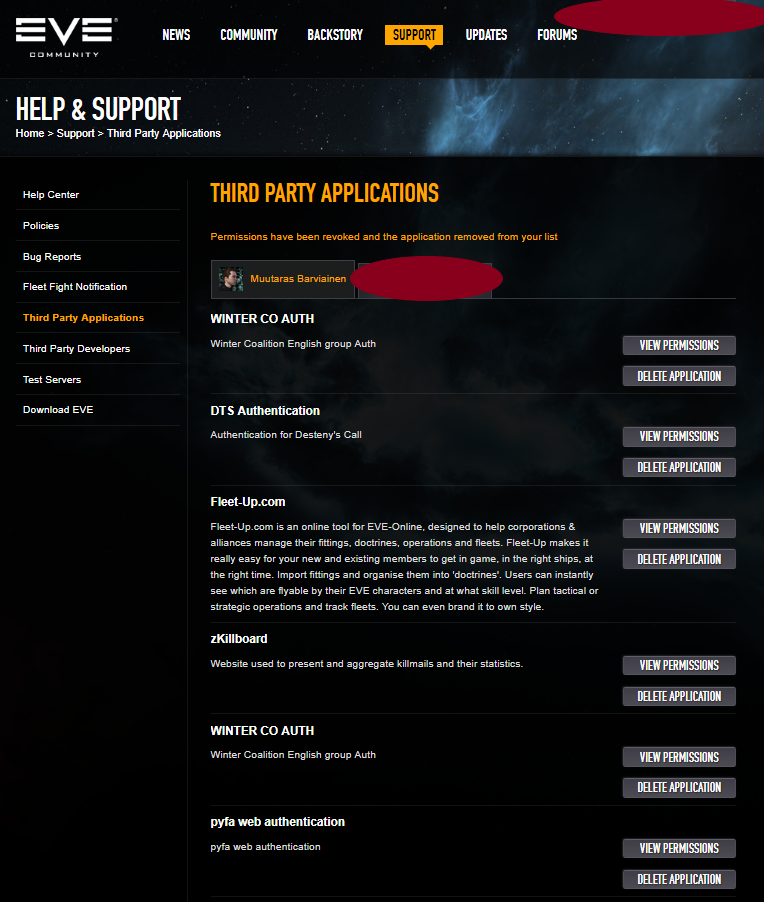
\includegraphics[scale=0.5]{APIs.png}